\chapter{Outlook} \label{chap:Outlook}
This chapter outlines important aspects that should be considered when further realizing an Ethernet-based implementation for a Distributed Test Support System.

\section{Implementation in the DML}
Since the investigations have shown that a UDP-based solution is feasible, the next step is to implement it in the DML (see \ref{chap:DML}). This will be done by the author after the thesis.

This involves replacing the FIFO buffers in the Data Management Layer for the remote nodes with UDP sockets. The Data Manager will then poll these sockets instead of the FIFO buffers. In addition, data transmission to remote nodes of the distributed test support system must also be implemented using sockets instead of DMA.

After implementation, extensive testing with the UDP-based DML solution should be performed.

\section{Detection of Network Overload}
According to the key results (see Section \ref{chap:KeyResults}), high network loads can have a negative impact on the reliability and performance of computer systems. To inform the user of the test support system that the system is operating at a load limit and degradation might be experienced, a network overlaod detection mechanism should be implemented.

This mechanism could be implemented in the Data Manager of the DML. A possible solution is to monitor the average throughput of all UDP communications of the system and to issue a warning message to the user at a certain threshold, which depends on the type of system.

\section{Fragmentation Algorithm based on UDP}
In the Distributed Test Support System, messages exchanged through the DML may exceed the maximum datagram size of the UDP protocol of 65,515 bytes. To transmit these messages using a UDP socket, a fragmentation algorithm must be implemented by the application.

Based on the results of the investigation that unfragmented UDP datagrams are not reordered in a local network without a switch, the information required for fragmentation and defragmentation can be significantly reduced compared to the IP protocol (see \ref{chap:frag}). A proposal for a fragmentation mechanism is outlined below.

\begin{figure}[h!]
    \centering
    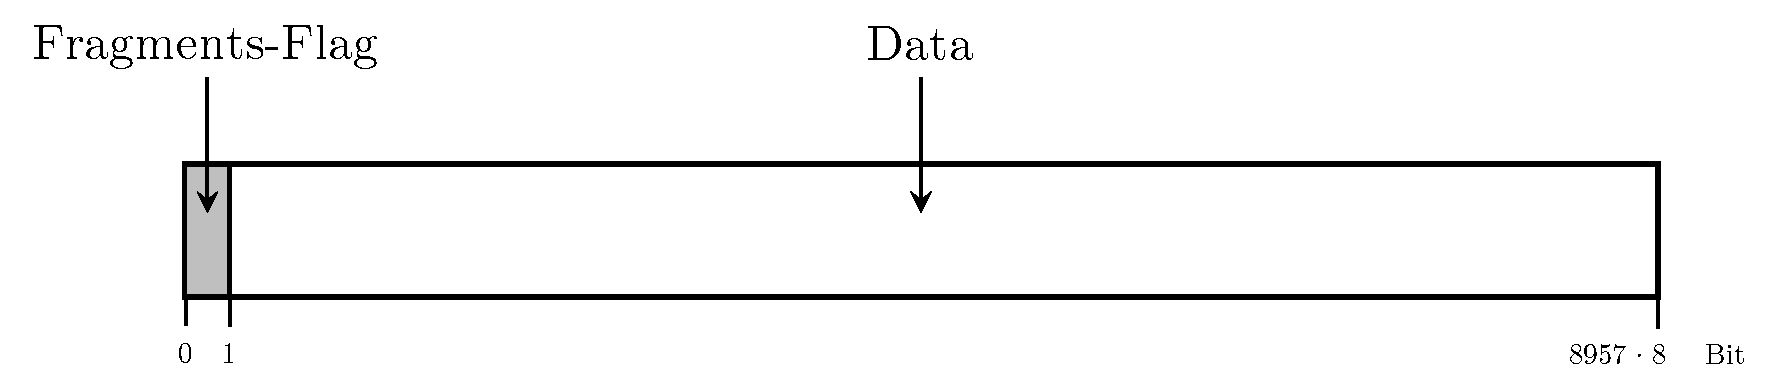
\includegraphics[width=1\linewidth]{figures/outlook/frag_header.pdf}
    \caption{Proposed Message Format for Implementation of a Fragmentation Mechanism}
    \label{fig:FragProposal}
\end{figure}

Figure \ref{fig:FragProposal} shows the proposed message format for the implementation of a fragmentation mechanism. A `Fragments-Flag' of 1 bit size is used. This is followed by the data. The maximum message size passed to the UDP socket is 8958 bytes, so no fragmentation is performed by the IP protocol with an MTU of 9000 bytes.

The 'Fragments-Flag' is not set for unfragmented messages. For fragmented messages, the 'Fragments-Flag' should be set for all fragments except the last one. This allows the recipient to identify the individual fragments and assemble them into a complete message. The absence of the flag on the last fragment indicates that all parts of the message have been received and defragmentation can be initiated.

\section{Reduction of Latency with DPDK}
DPDK (Data Plane Development Kit) is a collection of software libraries and drivers that enable the processing of network traffic directly in user space. This reduces latency and increases throughput by eliminating context switches between user space and kernel space, as well as the overhead of the standard Linux network stack \cite{outl02}.

Emmerich et al. found in \cite{outl01} that using the DPDK reduces latency compared to the standard Linux network stack. A substantial reduction was observed, especially in worst-case scenarios.